\documentclass[a4paper,14pt,oneside,final]{extarticle}
\usepackage[top=2cm, bottom=2cm, left=3cm, right=1cm]{geometry}
\usepackage{scrextend}

\usepackage[T2A,T1]{fontenc}
\usepackage[ukrainian,russian,english]{babel}
\usepackage{tempora}
\usepackage{fontspec}
\setmainfont{tempora}

% Зачем: Отключает использование изменяемых межсловных пробелов.
% Почему: Так не принято делать в текстах на русском языке.
\frenchspacing

\usepackage{indentfirst}
\setlength{\parindent}{1.25cm}
\renewcommand{\baselinestretch}{1.5}

% Header
\usepackage{fancyhdr}
\pagestyle{fancy}
\fancyhead{}
\fancyfoot{}
\fancyhead[R]{\small \selectfont \thepage}
\renewcommand{\headrulewidth}{0pt}

% Captions
\usepackage{chngcntr}
\counterwithin{figure}{section}
\counterwithin{table}{section}
\usepackage[tableposition=top]{caption}
\usepackage{subcaption}
\DeclareCaptionLabelFormat{gostfigure}{Рисунок #2}
\DeclareCaptionLabelFormat{gosttable}{Таблиця #2}
\DeclareCaptionLabelSeparator{gost}{~---~}
\captionsetup{labelsep=gost}
\captionsetup[figure]{labelformat=gostfigure}
\captionsetup[table]{labelformat=gosttable}
\renewcommand{\thesubfigure}{\asbuk{subfigure}}

% Sections
\usepackage[explicit]{titlesec}
\newcommand{\sectionbreak}{\clearpage}

\titleformat{\section}
  {\centering}{\thesection \quad}{0pt}{\MakeUppercase{#1}}
\titleformat{\subsection}[block]
  {\bfseries}{\thesubsection \quad #1}{0cm}{}

\titlespacing{\section} {0cm}{0cm}{21pt}
\titlespacing{\subsection} {\parindent}{21pt}{0cm}
\titlespacing{\subsubsection} {\parindent}{0cm}{0cm}

% Lists
\usepackage{enumitem}
\renewcommand\labelitemi{--}
\setlist[itemize]{noitemsep, topsep=0pt, wide}
\setlist[enumerate]{noitemsep, topsep=0pt, wide, label=\arabic*}
\setlist[description]{labelsep=0pt, noitemsep, topsep=0pt, leftmargin=2\parindent, labelindent=\parindent, labelwidth=\parindent, font=\normalfont}

% Toc
\usepackage{tocloft}
\tocloftpagestyle{fancy}
\renewcommand{\cfttoctitlefont}{}
\setlength{\cftbeforesecskip}{0pt}
\renewcommand{\cftsecfont}{}
\renewcommand{\cftsecpagefont}{}
\renewcommand{\cftsecleader}{\cftdotfill{\cftdotsep}}

\usepackage{float}
\usepackage{pgfplots}
\usepackage{graphicx}
\usepackage{multirow}
\usepackage{amssymb,amsfonts,amsmath,amsthm}
\usepackage{csquotes}

\usepackage{listings}
\lstset{basicstyle=\footnotesize\ttfamily,breaklines=true}
\lstset{language=Matlab}

\usepackage[
	backend=biber,
	sorting=none,
	language=auto,
	autolang=other
]{biblatex}
\DeclareFieldFormat{labelnumberwidth}{#1}

\lstdefinelanguage{CLIPS}{
  keywords={defrule, deftemplate},
  keywordstyle=\color{NavyBlue}\bfseries,
  emph={retract, modify, printout, assert, not},
  emphstyle={\color{OrangeRed}},
  identifierstyle=\color{black},
  sensitive=true,
  commentstyle=\color{gray}\ttfamily,
  comment=[l]{;;;},
}


\newcommand{\labnumber}{4} % fourth lab
\documentclass[a4paper,14pt,oneside,final]{extarticle}
\usepackage[top=2cm, bottom=2cm, left=3cm, right=1cm]{geometry}
\usepackage{scrextend}

\usepackage[T2A,T1]{fontenc}
\usepackage[ukrainian,russian,english]{babel}
\usepackage{tempora}
\usepackage{fontspec}
\setmainfont{tempora}

% Зачем: Отключает использование изменяемых межсловных пробелов.
% Почему: Так не принято делать в текстах на русском языке.
\frenchspacing

\usepackage{indentfirst}
\setlength{\parindent}{1.25cm}
\renewcommand{\baselinestretch}{1.5}

% Header
\usepackage{fancyhdr}
\pagestyle{fancy}
\fancyhead{}
\fancyfoot{}
\fancyhead[R]{\small \selectfont \thepage}
\renewcommand{\headrulewidth}{0pt}

% Captions
\usepackage{chngcntr}
\counterwithin{figure}{section}
\counterwithin{table}{section}
\usepackage[tableposition=top]{caption}
\usepackage{subcaption}
\DeclareCaptionLabelFormat{gostfigure}{Рисунок #2}
\DeclareCaptionLabelFormat{gosttable}{Таблиця #2}
\DeclareCaptionLabelSeparator{gost}{~---~}
\captionsetup{labelsep=gost}
\captionsetup[figure]{labelformat=gostfigure}
\captionsetup[table]{labelformat=gosttable}
\renewcommand{\thesubfigure}{\asbuk{subfigure}}

% Sections
\usepackage[explicit]{titlesec}
\newcommand{\sectionbreak}{\clearpage}

\titleformat{\section}
  {\centering}{\thesection \quad}{0pt}{\MakeUppercase{#1}}
\titleformat{\subsection}[block]
  {\bfseries}{\thesubsection \quad #1}{0cm}{}

\titlespacing{\section} {0cm}{0cm}{21pt}
\titlespacing{\subsection} {\parindent}{21pt}{0cm}
\titlespacing{\subsubsection} {\parindent}{0cm}{0cm}

% Lists
\usepackage{enumitem}
\renewcommand\labelitemi{--}
\setlist[itemize]{noitemsep, topsep=0pt, wide}
\setlist[enumerate]{noitemsep, topsep=0pt, wide, label=\arabic*}
\setlist[description]{labelsep=0pt, noitemsep, topsep=0pt, leftmargin=2\parindent, labelindent=\parindent, labelwidth=\parindent, font=\normalfont}

% Toc
\usepackage{tocloft}
\tocloftpagestyle{fancy}
\renewcommand{\cfttoctitlefont}{}
\setlength{\cftbeforesecskip}{0pt}
\renewcommand{\cftsecfont}{}
\renewcommand{\cftsecpagefont}{}
\renewcommand{\cftsecleader}{\cftdotfill{\cftdotsep}}

\newcommand{\khpistudentgroup}{КН-34г}
\newcommand{\khpistudentname}{Чепурний~А.~С.}

\newcommand{\khpidepartment}{Програмна інженерія та інформаційні технології управління}
\newcommand{\khpititlewhat}{
	Лабораторна робота №\labnumber \\
	з предмету <<Моделювання систем>>
}
\newcommand{\khpititlewho}{
	Виконав: \\
	\hspace*{\parindent} ст. групи \khpistudentgroup \\
	\hspace*{\parindent} \khpistudentname \\
	Перевірила: \\
	\hspace*{\parindent} ст. в. каф. ПІІТУ \\
	\hspace*{\parindent} Єршова~С.~І. \\
	\hspace*{\parindent} ас. каф. ПІІТУ \\
	\hspace*{\parindent} Литвинова~Ю.~С. \\
}



\lstset{language=CLIPS}
\graphicspath{{figures/}}

\begin{document}
\Ukrainian

\begin{titlepage}

\begin{center}
	МІНІСТЕРСТВО ОСВІТИ І НАУКИ УКРАЇНИ \\
	НАЦІОНАЛЬНИЙ ТЕХНІЧНИЙ УНІВЕРСИТЕТ \\
	«ХАРКІВСЬКИЙ ПОЛІТЕХНІЧНИЙ ІНСТИТУТ» \\[0.5cm]
	Кафедра <<\khpidepartment>> \\
\end{center}

\vspace{6cm}

\begin{center}
	\khpititlewhat
\end{center}

\vspace{3cm}

\begin{addmargin}[10cm]{0cm}
	\khpititlewho
\end{addmargin}

\vspace{\fill}

\begin{center}
	Харків \the\year
\end{center}

\end{titlepage}

\addtocounter{page}{1}

\section*{Розробка прототипу діагностичної експертної системи}
\subsection*{Мета}
\begin{enumerate}
	\item Сформувати для ПО поле знань, список фактів, а також правил для роботи з ними.
	\item Оволодіти базовими конструкціями мови представлення знань CLIPS, такими як deftemplate, deffacts, defrule, deffunction, defglobal.
	\item Освоїти принципи пошуку рішення в експертних системах, заснованих на правилах виду <<ЯКЩО-ТО>>, формування послідовності активації правил при виведенні результату.
\end{enumerate}

\subsection*{Завдання}
\begin{enumerate}
	\item Описати словесно факти і правила для розроблюваного прототипу, уявити можливу ієрархію понять. 
	\item Перекласти факти і правила в синтаксис мови CLIPS.
	\item Продемонструвати працездатність прототипу на конкретних прикладах.
\end{enumerate}

\begin{center}
Управління страховими договорами
\end{center}

\subsection*{Хід роботи}
Описати словесно факти і правила для розроблюваного прототипу, уявити можливу ієрархію понять.

Факти предметної області:
\begin{enumerate}
	\item \textbf{income}: low, normal, high; 
	\item \textbf{age}: young, mature, elderly;
	\item \textbf{status}: single, plural.
\end{enumerate}

Правила предметної області:
\begin{enumerate}
	\item \textbf{income} high якщо >20000, normal якщо >10000, інакше low; 
	\item \textbf{age} elderly якщо >60, mature якщо >45, інакше young;
	\item \textbf{status} plural якщо є родина, інакше single.
	\item Правило результату приведено у вигляді таблиці: \\
		\begin{tabular}{l|lll}
			\textbf{Do I need an insurance?} & \textbf{income} & \textbf{age} & \textbf{status} \\\hline 
			\textbf{No} & low & young & single \\ 
			\textbf{No} & normal & young & single \\ 
			\textbf{Yes} & high & young & single \\ 
			\textbf{No} & low & mature & single \\ 
			\textbf{Yes} & normal & mature & single \\ 
			\textbf{Yes} & high & mature & single \\ 
			\textbf{Yes} & low & elderly & single \\ 
			\textbf{Yes} & normal & elderly & single \\ 
			\textbf{Yes} & high & elderly & single \\ 
			\textbf{No} & low & young & plural \\ 
			\textbf{Yes} & normal & young & plural \\ 
			\textbf{Yes} & high & young & plural \\ 
			\textbf{Yes} & low & mature & plural \\ 
			\textbf{Yes} & normal & mature & plural \\ 
			\textbf{Yes} & high & mature & plural \\ 
			\textbf{Yes} & low & elderly & plural \\ 
			\textbf{Yes} & normal & elderly & plural \\ 
			\textbf{Yes} & high & elderly & plural \\ 
		\end{tabular}
\end{enumerate}

Демонстрацію працездатності прототипа на кенкретних прикладах представлено на рисунках~\ref{fig:test_1},~\ref{fig:test_2},~\ref{fig:test_3},~\ref{fig:test_4}.

\begin{figure}[H]
	\centering
	    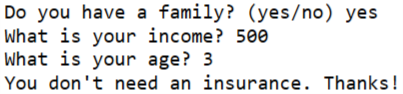
\includegraphics{test_1}
	\caption{Результат виконання програми №1}
	\label{fig:test_1}
\end{figure} 

\begin{figure}[H]
	\centering
	    
\includegraphics{test_2}
	\caption{Результат виконання програми №2}
	\label{fig:test_2}
\end{figure} 

\begin{figure}[H]
	\centering
	    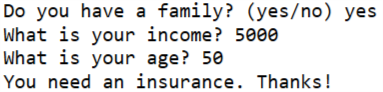
\includegraphics{test_3}
	\caption{Результат виконання програми №3}
	\label{fig:test_3}
\end{figure} 

\begin{figure}[H]
	\centering
	    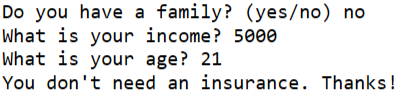
\includegraphics{test_4}
	\caption{Результат виконання програми №4}
	\label{fig:test_4}
\end{figure} 

\subsection*{Висновки}
У ході виконання лабораторної роботи я сформував для ПО поле знань, список фактів, а також правил для роботи з ними. 
Також я оволоділ базовими конструкціями мови представлення знань CLIPS, такими як deftemplate, deffacts, defrule, deffunction, defglobal. 
Я ознайомився з принципами пошуку рішення в експертних системах, заснованих на правилах виду "ЯКЩО-ТО", формування послідовності активації правил при виведенні результату.

\subsection*{Додаток}
Вихідний код програми:
\lstinputlisting{code/main.clp} 

\end{document}
